\documentclass[a4paper,10pt]{article}
%\usepackage[latin1]{inputenc} % Paquetes de idioma (otro encoding)
\usepackage[utf8]{inputenc} % Paquetes de idioma
\usepackage[spanish]{babel} % Paquetes de idioma
\usepackage{graphicx} % Paquete para ingresar gráficos
\usepackage{grffile}
\usepackage{hyperref}
\usepackage{fancybox}
\usepackage{amsmath}
\usepackage{amsfonts}
\usepackage{listings}
% Paquetes de macros de Circuitos
%\usepackage{pstricks}
\usepackage{tikz}

% Encabezado y Pié de página
\usepackage{fancyhdr} % Paquete para encabezados y pie de página
\pagestyle{fancy} % Sin esta línea no se imprimiría el encabezado en todas las páginas

\fancyhf{} %  Borra el encabezado anterior (Por defecto escribe el títutlo de la sección en la que se encuentra la hoja
\setlength{\headheight}{22.55pt}
\fancyhead[L]{
	{\textsf{Facultad de Ingenier\'ia $-$ Universidad de Buenos Aires \\ 66.09 Laboratorio de Microcomputadoras}}
}
%\addtocounter{page}{5}
\fancyhead[R]{\thepage}

\renewcommand{\footrulewidth}{0.4pt} % Ajusta el tamaño de las líneas separadoras en el pié de página
\renewcommand{\headrulewidth}{0.4pt} % Ajusta el tamaño de las líneas separadoras en el encabezado

\fancyfoot[L]{
	{\textsf{Anteproyecto} \\
	{\textsf{Integrantes: Torres Feyuk, Levi Hadid}}
	}
}
		

% Carátula del Trabajo
\title{ \author{} % Lo pongo para que el warning no moleste :p
\setlength{\unitlength}{1cm} %  Especifica la unidad de trabajo
\thispagestyle{empty}

\begin{picture}(18,0)
\put(0,0){
\includegraphics[width=1.5cm, height=3cm]{Imagenes/Logo1.png}}

\put(10.5,0){
\includegraphics[width=3cm, height=3cm]{Imagenes/Logo2.png}}

\end{picture}
\\[1.5cm]
\begin{center}
	\textbf{{\Huge Facultad de Ingenier\'ia \\ Universidad de Buenos Aires}}\\[2cm]
	{66.09 Laboratorio de Microcomputadoras}\\[0.5cm]
	{Anteproyecto}\\[2.5cm]
\end{center}

\begin{flushleft}
	\textbf{Integrantes:} \\[1cm]

	\begin{tabular}{|c|c|c|}
		\hline
		\textbf{\normalsize Padr\'on} & \textbf{\normalsize Nombre} & \textbf{\normalsize Email} \\
		\hline
		\normalsize 89579 & \normalsize Torres Feyuk, Nicol\'as R. Ezequiel & \normalsize ezequiel.torresfeyuk@gmail.com \\
		\hline
		\normalsize 90406 & \normalsize Levi Hadid, Lucas Alberto & \normalsize lucaslh9@hotmail.com \\
%		\hline
%		\normalsize ????? & \normalsize Madariaga, Eduardo & \normalsize madariagaedu@gmail.com \\
		\hline
	\end{tabular}
\end{flushleft}
\date{} % Hace que no se imprima la fecha en la cual se compilo el .tex
 }

\begin{document}
	\maketitle % Hace que el título anterior sea el principal del documento
	\newpage

	\tableofcontents % Esta línea genera un indice a partir de las secciones y subsecciones creadas en el documento
	\newpage

	\section{Objetivos}
		El objetivo del presente trabajo práctico consiste en diseñar e implementar un sistema que permita controlar los motores de un autito RC mediante 
		comunicación inalámbrica. 

	\section{Prestaciones Técnicas}
		\begin{itemize}
			\item El autito debe contar con 4 velocidades de funcionamiento, algo similar a una caja de cambios.
			\item La comunicación inalámbrica debe abarcar un rango máximo de 10 metros. 
			\item Se debe tener un control absoluto del auto a través del control remoto.
			\item Se debe alimentar tanto a la plaqueta del control como la del auto con baterias de 9V.
		\end{itemize} 

	\section{Descripción del Proyecto}
		El proyecto consiste en realizar el sistema de control de un auto de juguete el cual utiliza motores de continua para desplazarse, de forma tal de 
		manejar al mismo de forma remota a través de un control. Dado que lo que se desea es diseñar y construir el sistema y no la parte mecánica, se
		 utiliza en el presente proyecto  el chasis y los motores de un autito de juguete. \\
		\indent El vehículo a utilizar consta de dos motores de continua en las ruedas traseras del mismo. De esta forma, para lograr que el vehículo gire 
		tanto a la derecha como a la izquierda se debe alimentar a uno de los motores mientras el otro se mantiene fijo. Para lograr que el auto se desplace 
		para adelante o atrás solo basta con alimentar a los motores con la misma señal de forma que se muevan para el mismo lado y con la misma 
		potencia. \\
		\indent El auto será controlado a través de un control remoto que se encontrará enviando constantemente una señal al autito. Este último procesará 
		esta señal
		y según lo recibido se moverá en la dirección indicada y cambiará su velocidad a la indicada..	
	
		
	\section{Diagrama en Bloque}
		\subsection{Autito}
		\subsection{Control}
			
			\begin{figure}[!htb]
				\centering
				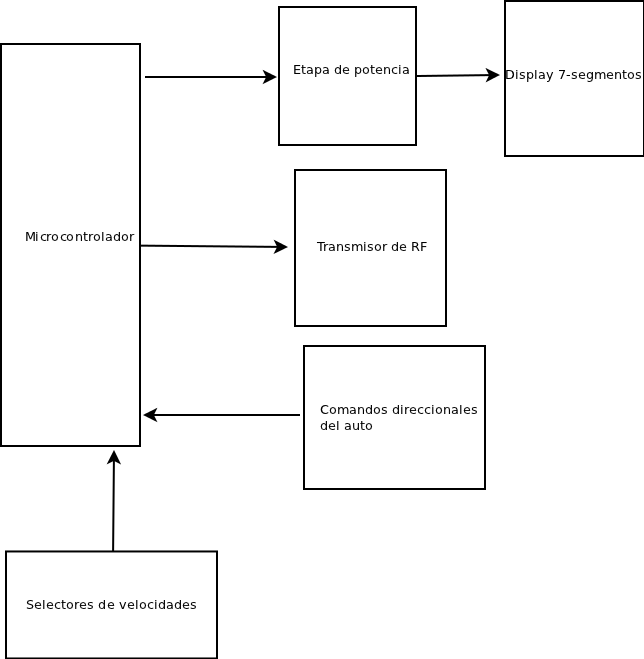
\includegraphics[width=11cm]{Imagenes/Diagrama1.png}
				\caption{Diagrama en Bloques del Control Remoto} \label{limg001}
			\end{figure}

	\section{Circuitos Esquemáticos}
		\subsection{Autito}
			\begin{figure}[!htb]
				\centering
				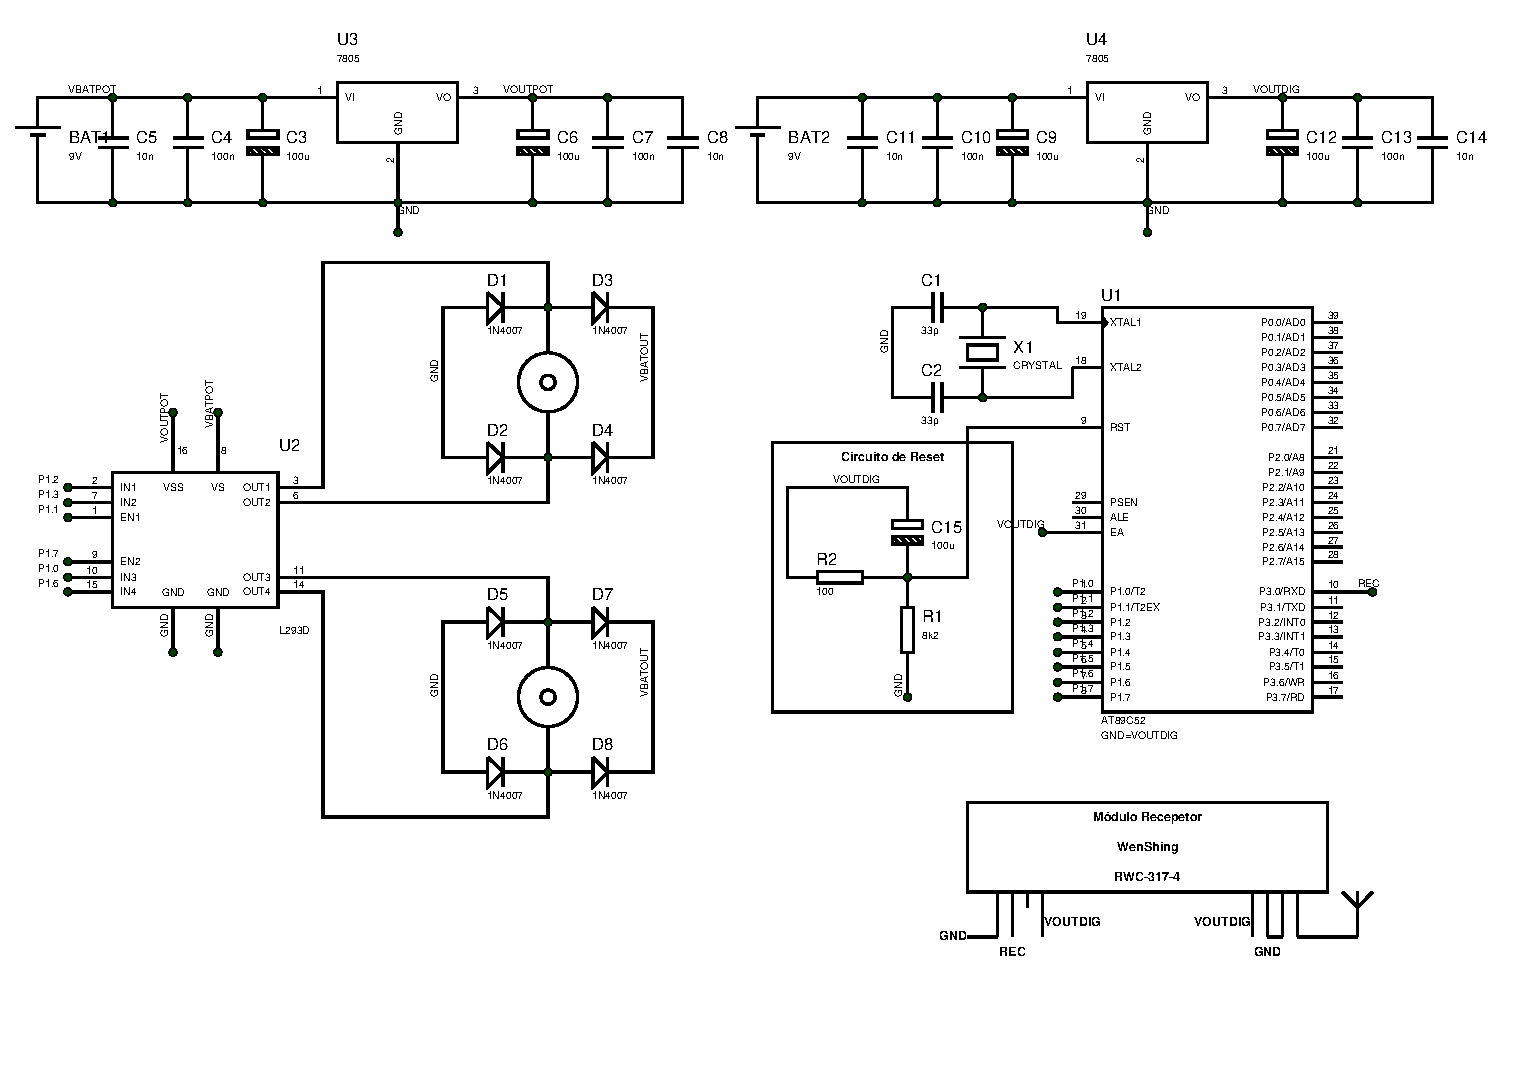
\includegraphics[width=11cm]{Imagenes/EsquematicoAuto.PDF}
				\caption{Diagrama en Bloques del Control Remoto} \label{limg003}
			\end{figure}
		
		\subsection{Control}
			La placa de control es alimentada con una batería de 9V. Se utiliza el
			dispositivo 7805 para adaptar la tensión de 9V entregada por la batería
			a una tensión de 5V necesaria para el funcionamiento del microcontrolador (AT89S52).
			El 7805 se inserta en el circuito acompañado de una configuración de capacitores de
			100uF, 100nF y 10nF, como puede observarse en la figura \ref{limg002}. Estos 						capacitores cumplen la función de estabilizar la tensión de alimentación en VCC=5V para 			que no haya oscilaciones indeseables de tensión respecto del valor requerido.
			La pata de VCC del microcontrolador AT89S52 es conectada a los 5V obtenidos de
			la pata de VCC de salida del 7805, y de esta forma se alimenta al microcontrolador. 				También se conecta la pata EA del microcontrolador a VCC para que el micro utilice la 				ROM interna para código. Entre los terminales XTAL1 y XTAL2 se conecta un cristal de 				11.059MHz de la forma en que se muestra en la figura \ref{limg002}.\\
			\indent En la figura podemos ver también el circuito de reset utilizado. Este se 					conecta a la pata RST del microcontrolador y consta de una resistencia de 100$\Omega$, 				una de 8.2k$\Omega$, un capacitor de 100uF y un pulsador. Al apretar el pulsador, la 				pata RST del micro se pone en estado alto hasta que éste deje de ser pulsado. El 					capacitor hace que se mantenga en estado alto esta pata durante el tiempo necesario 				para que el micro se termine de resetar.\\
			\indent Todos los puertos del microcontrolador, a excepción del puerto 0, tienen una 
			red de pull-up que permite trabajar con estos puertos sin necesidad de utilizar una 				alimentación externa (ya que internamente, cada uno de los pines del puerto está 					conectado a VCC a través de una resistencia de pull-up).\\
			\indent Se utilizó el puerto 2, más especificamente las patas P2.0, P2.1, P2.2 y P2.3,
			como los terminales del microcontrolador a través de los cuales se ingresan los 					de comandos de dirección que controlarán el autito. Estos comandos son ingresados al 				micro a través de 4 pulsadores, uno para cada dirección (adelante, atrás, izquierda, 				derecha). Cada véz que se presionan los pulsadores, se conecta las correspondientes 				patas del puerto a GND, lo que hace que se escriba un 0 en éstas. De esta forma, el 				micro actuará de la forma adecuada en concordancia con la entrada ingresada.
			\indent A las patas de interrupciones INT0 e INT1 se conectan 2 pulsadores que se 					utilizarán para cambiar las velocidades. Estos pulsadores son conectados de la misma 				forma que aquellos que controlan las direcciones del autito.\\
			\indent El puerto 1 se utiliza para controlar un display 7-segmentos que se encarga de 				mostrar la velocidad a la que está funcionando el autito. Como el puerto es incapaz de 				entregar la potencia necesaria para hacer funcionar correctamente el display de
			7-segmentos, se conecta como etapa intermedia entre el microcontrolador y el display, 				una etapa de potencia proporcionada por el dispositivo ULN2803, qué basicamente es un 				array de transistores que se encarga de aumentar la corriente entrante al display 					(corriente que el microcontrolador es incapaz de entregar por sí solo).\\
			\indent En la figura \ref{limg002} se puede ver la forma de conexionado entre el 					microcontrolador, el ULN2803, y el display 7-segmentos.El ULN2803 tiene varias entradas
			y salidas (una entrada-salida para cada pata del puerto correspondiente con cada
			led) y una pata de GND que se conecta a la masa del circuito. Entre el ULN2803 y el
			display,se colocaron, en cada una de las lineas correspondientes a cada led del
			display, resistencias de 270$\Omega$ para limitar la corriente que circula por cada led
			y evitar,de esta forma, que los mismos se quemen. Las patas del puerto del micro se
			conectan a las entradas del ULN2803, como puede verse en la fugra \ref{limg002}.Se
			agregaron resistencias de 2.7k$\Omega$ entre las patas del puerto y VCC de manera tal 				de generar una resistencia de pull-up equivalente menor (resultado del paralelo entre 				la resistencia de pull-up interna del micro y la resistencia agregada), que le permita
			al micro entregar una mayor corriente necesaria para alimentar al ULN2803, y conseguir 				de esta forma el correcto funcionamiento del display 7-segmentos.\\
			\indent Para la transmisión RF, se uso el módulo TWS-BS3. Este módulo cuenta con 4 					patas: una que se conecta a VCC, otra que se conecta a GND, otra que recibe 						la información digital proveniente del puerto serie del micro, más específicamente de
			la pata TXD, y una última pata que es la que se conecta a la antena necesaria para 					transmitir.\\
			
			
			
			
			\begin{figure}[!htb]
				\centering
				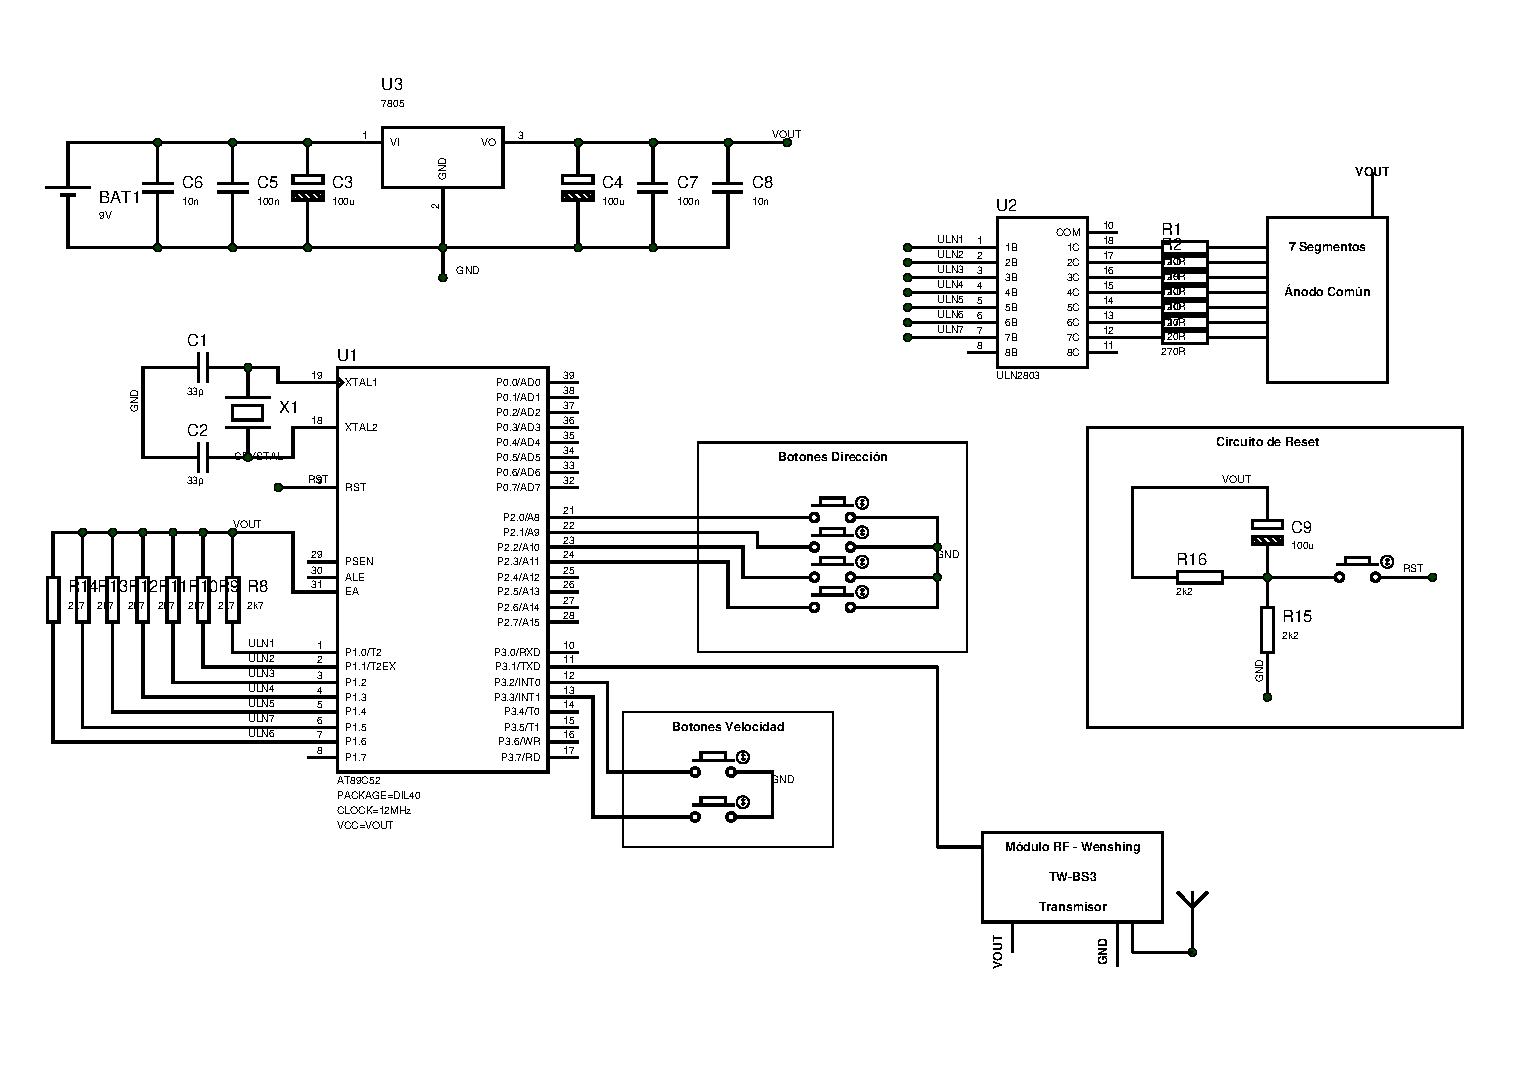
\includegraphics[width=11cm]{Imagenes/EsquematicoControl.PDF}
				\caption{Circuito esquematico del Control Remoto} \label{limg002}
			\end{figure}
	
	\section{Listado de Componentes}
	
		\begin{tabular}{|c|c|c|}
		\hline
		\textbf{\normalsize Componente} & \textbf{\normalsize Precio unitario} & 							\textbf{\normalsize Cantidad} \\
		\hline
		Placas experimentales 10cm X 10cm & & 2\\
		\hline
		Placas experimentales 10cm X 5cm & & 1\\
		\hline
		Baterías de 9V & & 3\\
		\hline
		AT89S52 & & 2\\
		\hline
		TWS-BS3 & & 1\\
		\hline
		RWS-371-4 & & 1\\
		\hline
		7805 & & 3\\
		\hline
		L293D & & 1\\
		\hline
		ULN2803 & & 1\\
		\hline
		Cristales 11.059MHz & & 2\\
		\hline
		Diodos & & 8\\
		\hline
		Pulsadores & & 8\\
		\hline
		Capacitores 3 pF & & 5\\
		\hline
		Capacitores 10 nF & & 8\\
		\hline
		Capacitores 100 nF & & 7\\
		\hline
		Capacitores 10 uF & & 2\\
		\hline
		Capacitores 100 uF &  & 7\\
		\hline
		Resistencias 100$\Omega$ & & 2\\
		\hline
		Resistencias 270$\Omega$ - 5\% & & 7\\
		\hline
		Resistencias 2.7k$\Omega$ - 5\% & & 7\\
		\hline
		Resistencias 8.2k$\Omega$ - 5\% & & 2\\
		\hline
		Zócalos - 40 patas & & 2\\
		\hline
		Zócalos - 9 patas & & 1\\
		\hline
		Zócalos - 8 patas & & 1\\
		\hline
		\end{tabular}
	\section{Software}
	\section{Resultados}
	\section{Conclusiones}

\end{document}
